{
Denne udvidelse sigter mod at forbedre den eksisterende bedømmelse af
interessante regioner i forhold til det gyldne snit. Specielt er der
en type af interessante regioner som bliver fravalgt af den naive
metode, nemlig regioner med massemidtpunkt i det gyldne snit, men med et
afgrænsende rektangel uden for margin. Et eksempel på dette kan ses i
figur \ref{hus}, hvor den sorte region ikke anses som liggende i det
gyldne snit af den naive fremgangsmåde. Vi vil gerne have at sådanne
regioner klassificeres som en positiv interessant region.

% Original
%I denne udvidelse vil vi gerne indføre mere udføliger defination af
%hvornår en ragion ligger i et snit. hvor vi før kun arbejdet med
%ragionen som tagenteret inde i snittet, vil vi nu også gerne have
%ragioner med som skæres i midden af snittet se figur
%\ref{hus}.

\begin{figure}[h]
	\begin{center}
		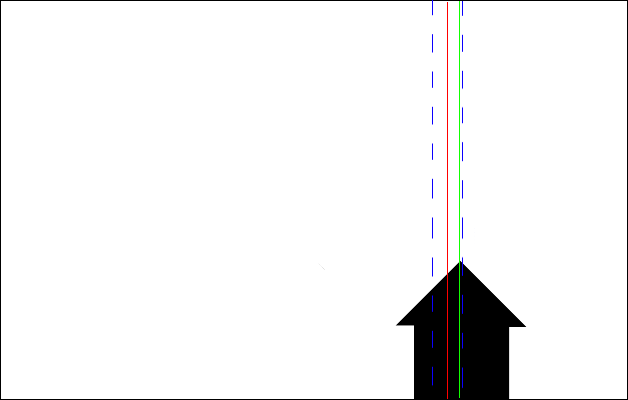
\includegraphics[scale=0.3,angle=0]{afsnit/vores_implementation/billeder/udvidet_loesning/husworks.png}
	\end{center}
	\caption[]{Et hus som bliver skåret over i midden af snittet}
	\label{hus}
\end{figure}

% Dette er implementations-snak! Det kan dog godt nævnes hurtigt.
% Det er langt vigtigere at høre om metoden med det samme.

%\subsubsection{Opdeling af ragion med et grid}
%Når vi

% Original
%\subsubsection{Opdeling af ragion med et grid}
%Måden vi deller ragionen op på, er hved hjælp af et gridt som vi
%tilføjer vær baunding box, se figur \ref{grid}. Da vi ved hvilken farve
%baunding boxens ragion er, tager vi alle de punkter i grittet som har
%denne farve, og få der ved en bedre beskrivels af hvordan ragionen ser
%ud. For at gøre algoritmen lidt hurtiger, er vores gridt punkter lavet
%med 2 pixels mellemrum. XXX(dette rette vi nå vi pracis ved hvor stort
%vores gridt er) XXX(har vi skravet at vi altid laver ragionerne
%forskelige farver.)

%\begin{figure}[h]
%	\begin{center}
%		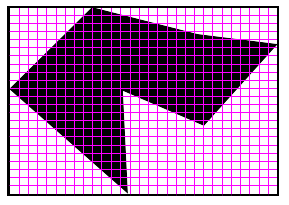
\includegraphics[scale=0.76,angle=0]{afsnit/vores_implementation/billeder/udvidet_loesning/udvidetloesninglayer.png}
%	\end{center}
%	\caption[]{Et grid over en ragion i baunding box}
%	\label{grid}
%\end{figure}

\subsubsection{Bedømmelse med hensyn til massemidtpunkt}
Givet en region $R$ betegner vi antallet af punkter i regionen med
$|R|$. Vi antager at vi betragter et vertikalt snit $G$ i et billede.
Det gælder for alle punkter $p \in R$ at de kan befinde sig ovenpå, til
højre eller til venstre for $G$. I denne sammenhæng lader vi $R_r$ og
$R_l$ beskrive punkter henholdsvis til højre og venstre for snittet $G$.
Afstanden fra et punkt til snittet $G$ betegner vi $d$, mens afstanden
fra en punkt til kanten af et billede kaldes $D$. Med disse
informationer kan vi afgøre om regionen bliver delt i to lige store dele
af snittet samt om store dele af regionen befinder sig langt væk fra
snittet. Vi definerer nu to funktioner som kan sige noget om regionens
form.

%Vi har nu x antal punkter i en ragion og vi andtager at det er et af den
%vertikale snit vi ser på. Så kan punkterne befinde sig oven på snittet,
%til venstre eller til højre fra snittet. Alle punkterne har også en
%afstand d til snittet og en afstand D til kanten af billedet. Med de 3
%information kan vi sige en masse om ragionen, f.eks. skære snitte
%ragionen i 2 lige store delle eller befinder næste helle figuren sig
%lang væk fra snittet osv. Få at få nogle konkrate matematik ned, har vi
%valt at se på disse 2 formler
%\ref{MPunkt}, \ref{Fordeling}.

\begin{eqnarray}
    m(R) & = & \frac{\sum_{p \in R}{D}}{|R|}
    \label{MPunkt}
\end{eqnarray}
\begin{eqnarray}
    f(R) & = & \frac{|R_{l}| - |R_{r}|}{|R|}
    \label{Fordeling}
\end{eqnarray}
%\begin{eqnarray}
% MPunkt &=& \frac {\sum{D}}{x}\label{MPunkt}
%\end{eqnarray}

%\begin{eqnarray}
% Fordeling &=& \frac{x_{venstre~side}-x_{højre~side}}{x}\label{Fordeling}
%\end{eqnarray}

Formel \ref{MPunkt} finder et mid punktet af ragionen i forhold til
venstre side for vertikale snit og toppen ved højesuntale snit. se figur
\ref{midpunkt}

\begin{figure}[h]
	\begin{center}
		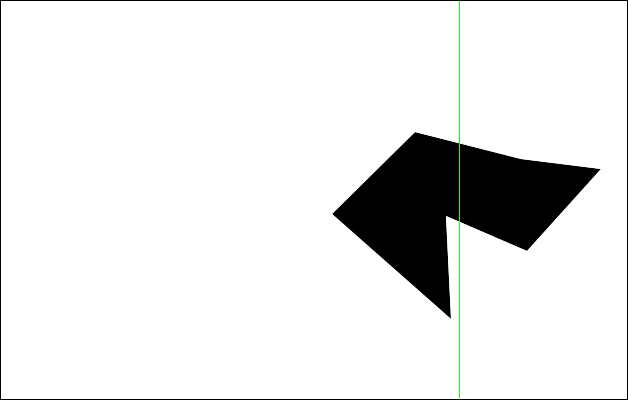
\includegraphics[scale=0.5,angle=0]{afsnit/vores_implementation/billeder/udvidet_loesning/centerOfmass.png}
	\end{center}
	\caption[]{ragion hvor masse midpunktet er tegnet in i forhold til venster side af billedet}
	\label{midpunkt}
\end{figure}

Vi sammen linier nu midpunktet med snittet og få en afstand, hvis denne
afstand er mindre en magien, så er ragione godtaget, se figur
\ref{cOMCutMargin}

\begin{figure}[h]
	\begin{center}
		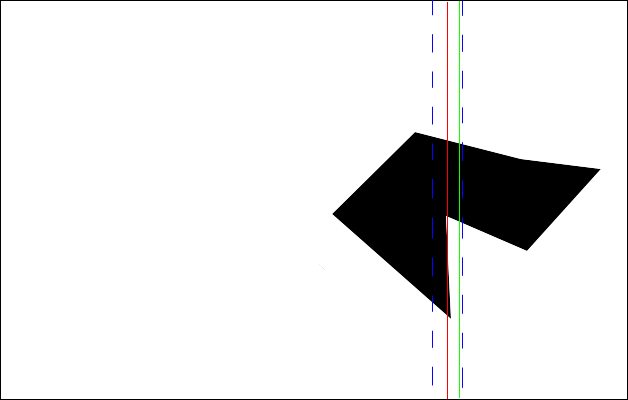
\includegraphics[scale=0.5,angle=0]{afsnit/vores_implementation/billeder/udvidet_loesning/cOMCutMargin.png}
	\end{center}
	\caption[]{ragion hvor masse midpunktet, snit og margin er teget ind, som man kan se ligger midpunktet inde for marginen}
	\label{cOMCutMargin}
\end{figure}

Nu skulle man tror at alting er godt men desværre kan vi kommer ud for
nogle figure som formel \ref{MPunkt} ikke tager højte for.

\begin{figure}[h]
	\begin{center}
		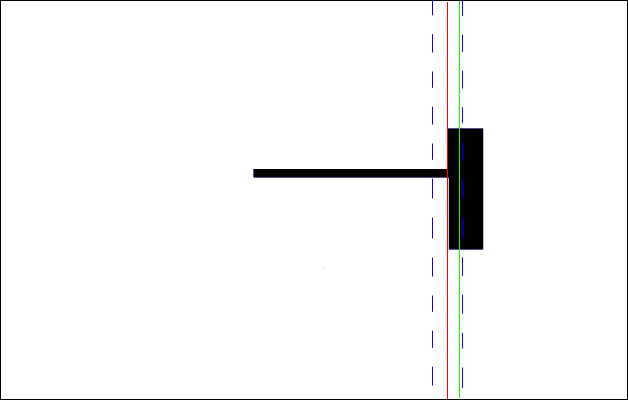
\includegraphics[scale=0.5,angle=0]{afsnit/vores_implementation/billeder/udvidet_loesning/dontWork.png}
	\end{center}
	\caption[]{Figur som overhold farmel \ref{MPunkt} men ikke \ref{Fordeling}}
	\label{dontwork}
\end{figure}

Som man kan se i figur \ref{Fordeling} er det fundene midpunkt inde for
marginen, men figur \ref{dontwork} har en lang stang som ænder med at
være lang væk fra snittet. Dette vil vi helt undgå da denne figur ikke
ligger i snittet. Men da de fleste pixels ligger på højre sider af
figuren kan vi, kan vi sotere denne figur væk ved at sammen line pixel
andtal på begge sider og se om den reletive pixeltal kommer under en vis
granse. Formel \ref{Fordeling} bruges til dette formål. Denne metode gør
også at vi få soteret de figure væk hvor snittet gå i gemmen side af
figuren, f.eks. et andsigt hvor snittet gå i gemmen kinden og ikke
næsen. se figur \ref{dontwork2}

\begin{figure}[h]
	\begin{center}
		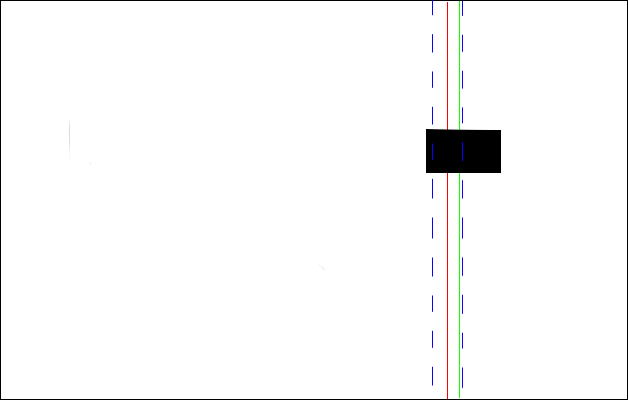
\includegraphics[scale=0.5,angle=0]{afsnit/vores_implementation/billeder/udvidet_loesning/dontwork2.png}
	\end{center}
	\caption[]{Figur som overhold farmel \ref{MPunkt} men ikke \ref{Fordeling}}
	\label{dontwork2}
\end{figure}

ud fra disse opsavatione, har vi indført de 3 kategoriera neden for.
kategori 1: Alle de ragioner som vi fand før med bounding box og $ |snit - MPunkt| \leq Q \wedge |Fordeling| \leq P_1$ \\
kategori 2: $|snit - MPunkt| \leq Q \wedge |Fordeling| \leq P_2 \wedge (snit - MPunkt)*fordeling \geq 0$ \\
kategori 3: Resten\\

Hvor Q er antal pixels mellem snittet og margien og $P_1$ og $P_2$ er procentvis forskel på de to sider.
Som man kan se vægter vi formlel \ref{MPunkt} højre en \ref{Fordeling}


\subsubsection*{brugbarhed}
\subsubsection*{Fordele vs ulember}

}

% vim: set tw=72 spell spelllang=da:
